\documentclass[12pt]{article}

\title{\vspace{-3em}PHYS 167b Exam 1}
\author{Michael Cardiff}
\date{\today}

%% science symbols
\usepackage{amsmath}
\usepackage{amssymb}
\usepackage{amsthm}
\usepackage{bm}
\usepackage{cancel}
\usepackage{physics}
\usepackage{siunitx}
\usepackage{slashed}

%% general pretty stuff
\usepackage{caption}
\usepackage{float}
\usepackage{graphicx}
\usepackage{url}
\usepackage{enumitem}
\usepackage{hyperref}
\usepackage{tikz}
\usepackage{tikz-feynhand}
\usepackage[margin=1in]{geometry}

% setup options
\captionsetup{labelfont=bf}
\graphicspath{ {./figs/} }

% macros
\renewcommand{\L}{\mathcal{L}}
\renewcommand{\H}{\mathcal{H}}
\renewcommand{\l}{\ell}
\renewcommand{\bar}{\overline}
\newcommand{\M}{\mathcal{M}}
\newcommand{\mcV}{\mathcal{V}}
\newcommand{\D}{\partial}
\newcommand{\veps}{\varepsilon}
\newcommand{\circled}[1]{\tikz[baseline = (char.base)]{
    \node[shape=circle,draw,inner sep=2pt] (char){#1};}}

% mdframed environments
\usepackage[framemethod=TikZ]{mdframed}
\mdfsetup{skipabove=\topskip,skipbelow=\topskip}
\mdfdefinestyle{defstyle}{%
  linewidth=1pt,
  frametitlerule=true,
  frametitlebackgroundcolor=gray!40,
  backgroundcolor=gray!20,
  innertopmargin=\topskip}

\mdtheorem[style=defstyle]{definition}{Definition}
\mdtheorem[style=defstyle]{theorem}{Theorem}
\mdtheorem[style=defstyle]{problem}{Problem}

\newenvironment{thebook}
{\begin{mdframed}[style=defstyle,frametitle={From the Book}]}{\end{mdframed}}

\usepackage{fancyhdr}

\usepackage{siunitx}
\DeclareSIUnit\barn{b}
\setlength{\feynhanddotsize}{0.01sp}
\usepackage{textcomp}
\pagestyle{fancy}
\makeatletter
\def\section{\@startsection{section}{1}{\z@ }%
  {-3.5ex\@plus -1ex\@minus -.2ex}{2.3ex \@plus .2ex}%
  {\noindent\normalfont \Large \bfseries Task\ }%
}
\makeatother
\lhead{Michael Cardiff}
\rhead{PHYS 167b Exam 1}
\numberwithin{equation}{section}

\begin{document}
% \maketitle
\section{Higgs Pair Production}
\begin{problem}
  The Higgs boson pair production process is used at the LHC to search for the Higgs trilinear self interaction (HHH) as shown in Figure~\ref{fig:t1}. The production cross section  is about $\SI{36.7}{fb}$ at $\sqrt{s}=\SI{14}{TeV}$.
  \begin{figure}[H]
    \centering
    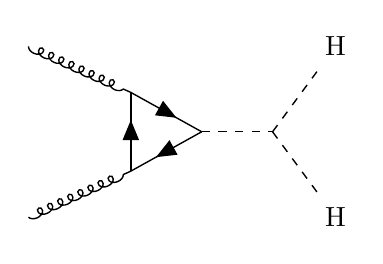
\begin{tikzpicture}
      \begin{feynhand}
        % vertices
        \vertex (g1) at (0,0);
        \vertex (g2) at (0,-2.17);
        \vertex (h1) at (3.9,0) {$\mathrm{H}$};
        \vertex (h2) at (3.9,-2.17) {$\mathrm{H}$};
        \vertex (a) at (1.3,-0.585);
        \vertex (b) at (1.3,-1.585);
        \vertex (c) at (2.2,-1.085);
        \vertex (d) at (3.1,-1.085);
        % propags
        \propag[glu] (g1) to (a);
        \propag[glu] (g2) to (b);
        \propag[sca] (d) to (h2);
        \propag[sca] (d) to (h1);
        \propag[sca] (c) to (d);
        % box
        \propag[antfer] (a) to (b);
        \propag[fer] (a) to (c);
        \propag[antfer] (b) to (c);
      \end{feynhand}
    \end{tikzpicture}
    \hspace{4em}
    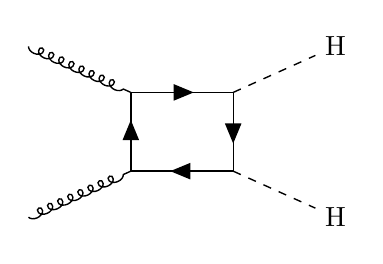
\begin{tikzpicture}
      \begin{feynhand}
        % vertices
        % externals
        \vertex (g1) at (0,0);
        \vertex (g2) at (0,-2.17);
        \vertex (h1) at (3.9,0) {$\mathrm{H}$};
        \vertex (h2) at (3.9,-2.17) {$\mathrm{H}$};
        % internals
        \vertex (a) at (1.3,-0.585);
        \vertex (b) at (1.3,-1.585);
        \vertex (c) at (2.6,-0.585);
        \vertex (d) at (2.6,-1.585);
        % propags
        \propag[glu] (g1) to (a);
        \propag[sca] (c) to (h1);
        \propag[glu] (g2) to (b);
        \propag[sca] (d) to (h2);
        % box
        \propag[antfer] (a) to (b);
        \propag[fer] (c) to (d);
        \propag[fer] (a) to (c);
        \propag[antfer] (b) to (d);
      \end{feynhand}
    \end{tikzpicture}
    \caption{Higgs pair production at the LHC}\label{fig:t1}
  \end{figure}
  \begin{enumerate}
  \item How many Higgs boson pair events  will be produced by the end of the High-Luminosity LHC with an integrated luminosity of $\SI{3}{ab^{-1}}$?
  \item There are a number of final states that can be studied depending on the Higgs boson  decays. From the given branching ratios in Table 17.1 of the textbook find the branching ratios to $bbbb$, $bb\gamma\gamma$, $bb\tau\tau$, and $bb\mathrm{WW}$ channels
  \item For Phys 167B:\@ What are the advantages and disadvantages for searching for $\mathrm{HH}$ in each of those channels? Explain.
  \end{enumerate}
\end{problem}
In order to calculate the number of events, we only need the cross section as well as the integrated luminosity:
\begin{thebook}
  The number of events of a certain type with cross section $\sigma$ and instantaneous luminosity $\L$ is given by:
  \begin{align*}
    N=\sigma\int\L\dd{t}
  \end{align*}
\end{thebook}
Then plugging in our numbers:
\begin{align*}
  N=\SI{36.7}{fb}\times\frac{\SI{1000}{ab}}{\SI{1}{fb}}
  \times\SI{3}{ab^{-1}}
\end{align*}
Giving our answer of:
\begin{equation}
  \label{eq:t11}
  \boxed{N_{\mathrm{H}\text{ pairs}}\approx 110100}
\end{equation}
For each of these final states, we need each of the Higgs to decay, so the total $BR$ will be the product of the two separate $BR$s:
\begin{itemize}
\item $bbbb$ requires both to decay to $b$ pairs:
  \begin{equation}
    \label{eq:t121}
    \boxed{BR(\mathrm{HH}\to bbbb)=BR{(\mathrm{H}\to bb)}^2\approx33\%}
  \end{equation}
\item $bb\gamma\gamma$ requires one $b$ pair and then a $\gamma$ pair, and from now on we need to take into account that there are two ways for a $bbXX$ state, if we assign labels to each $\mathrm{H}$, we have $\mathrm{H}^{(1)}\to bb,\mathrm{H}^{(2)}\to XX$ as well as $\mathrm{H}^{(1)}\to XX,\mathrm{H}^{(2)}\to bb$
  \begin{equation}
    \label{eq:t122}
    \boxed{BR(\mathrm{HH}\to bb\gamma\gamma)=
      2BR(\mathrm{H}\to bb)\times BR(\mathrm{H}\to\gamma\gamma)\approx0.23\%}
  \end{equation}
\item $bb\tau\tau$ requires one $b$ pair and then a $\gamma$ pair
  \begin{equation}
    \label{eq:t123}
    \boxed{BR(\mathrm{HH}\to bb\tau\tau)=
      2BR(\mathrm{H}\to bb)\times BR(\mathrm{H}\to\tau\tau)\approx7.40\%}
  \end{equation}
\item $bb\mathrm{WW}$ requires one $b$ pair and then a $\gamma$ pair
  \begin{equation}
    \label{eq:t124}
    \boxed{BR(\mathrm{HH}\to bb\mathrm{WW})=
      2BR(\mathrm{H}\to bb)\times BR(\mathrm{H}\to\mathrm{WW})\approx25.0\%}
  \end{equation}
\end{itemize}
There are several advantages and disadvantages to each of these states:
\begin{itemize}
\item $bbbb$
  \begin{itemize}
  \item Advantage: High $BR$, so large amount of statistics available
  \item Disadvantage: In order to find these states, need to distinctly identify 4 jets and ensure they are from $b$ quarks, which is highly nontrivial
  \end{itemize}
\item $bb\gamma\gamma$
  \begin{itemize}
  \item Advantage: $\gamma\gamma$ is a clean signal, and identifying dijet is much easier than 4
  \item Disadvantage: Extremely low $BR$
  \end{itemize}
\item $bb\tau\tau$
  \begin{itemize}
  \item Advantage: The $BR$ is not too large, but the higher mass of $\tau$ is advantageous here
  \item Disadvantage: Large background from $\mathrm{Z}\to\tau\tau$, and since the tau decays often include $\nu$ pairs, good measurements of $E^{miss}$ is required
  \end{itemize}
\item $bb\mathrm{WW}$
  \begin{itemize}
  \item Advantage: $\mathrm{W}$ has several final states, so low $BR$ is made up for by several identification methods
  \item Disadvantage: $\mathrm{W}$ production cross section is $\order{\unit{nb}}$ so very high background
  \end{itemize}
\end{itemize}
\newpage
\section{Breit-Wigner Resonance}
\begin{problem}
  A narrow resonance appears in $e^+e^-$  annihilation experiments at the center of mass energy of $\SI{9.5}{GeV}$. The resonance decays to both $\mu^+\mu^-$ as well as to hadrons. The measurements of the integrated cross sections yield:
  \begin{align*}
    \int\sigma_{\mu\mu}(E)\dd{E}&=\SI{8.5e-33}{cm^2MeV}\\
    \int\sigma_{\text{hadrons}}(E)\dd{E}&=\SI{3.3e-31}{cm^2MeV}
  \end{align*}

  Use the Breit-Wigner resonance formula to determine the partial widths $\Gamma_{\mu\mu}$ and $\Gamma_{\text{hadrons}}$ for the $\mu\mu$ and hadronic decays of the resonance. The so called non-relativistic Breit-Wigner can be used for this problem:\@ $\sigma=\frac{3\pi}{4M^2}\frac{\Gamma_i\Gamma_f}{{(E-M)}^2+\frac{\Gamma^2}4}$ and after performing the integral use the assumption that $\Gamma\ll M$. Assume lepton universality as the resonance can decay to electrons, muons, and taus. Give the answers in units of \unit{MeV}.
\end{problem}
Since the form of the cross section is identical in both cases we can simply perform the integral over $E$ generally before moving on to solve for anything:
\begin{align*}
  \int\sigma\dd{E}&=\frac{3\pi\Gamma_i\Gamma_f}{4m^2}
  \int_0^\infty\frac{\dd{E}}{{(E-m)}^2+\Gamma^2/4}\\
  &=\frac{3\pi}{2m^2}\frac{\Gamma_i\Gamma_f}{\Gamma}
  \int_{-2m/\Gamma}^\infty\frac{1}{u^2+1}\dd{u}\\
  &=\frac{3\pi}{2m^2}\frac{\Gamma_i\Gamma_f}{\Gamma}
  \eval{\arctan(u)}_{-2m/\Gamma}^\infty
\end{align*}
Where the substitution $u=2(E-m)/\Gamma$ was employed.

Since we have $\Gamma\ll m$, the lower limit turns into a $-\infty$:
\begin{align*}
  \frac{3\pi}{2m^2}\frac{\Gamma_i\Gamma_f}{\Gamma}
  \eval{\arctan(u)}_{-\infty}^\infty=
  \frac{3\pi^2}{2m^2}\frac{\Gamma_i\Gamma_f}{\Gamma}
\end{align*}
We then have the analytic values for the following integrals:
\begin{align*}
  \int\sigma_{\mu\mu}(E)\dd{E}&=
  \frac{3\pi^2}{2m^2}\frac{\Gamma_{ee}\Gamma_{\mu\mu}}{\Gamma}\\
  \int\sigma_{\text{hadrons}}(E)\dd{E}&=
  \frac{3\pi^2}{2m^2}\frac{\Gamma_{ee}\Gamma_{\text{hadrons}}}{\Gamma}
\end{align*}
Assuming the mystery particle can only decay hadronically and leptonically, as well as lepton universality, the total width would be given by:
\begin{align*}
  \Gamma=3\Gamma_{\mu\mu}+\Gamma_{\text{hadrons}}
\end{align*}
We can find an immediate relation between the two desired widths by taking the ratio of the two integrals:
\begin{align*}
  \frac{\int\sigma_{\mu\mu}(E)\dd{E}}{\int\sigma_{\text{hadrons}}(E)\dd{E}}
  &=\frac{\Gamma_{\mu\mu}}{\Gamma_{\text{hadrons}}}=\frac{c_1}{c_2}\\
  \implies\Gamma_{\text{hadrons}}&=\frac{c_2}{c_1}\Gamma_{\mu\mu}
\end{align*}
Where we have used the shorthand:
\begin{align*}
  \int\sigma_{\mu\mu}(E)\dd{E}&=\SI{8.5e-33}{cm^2MeV}\equiv c_1\\
  \int\sigma_{\text{hadrons}}(E)\dd{E}&=\SI{3.3e-31}{cm^2MeV}\equiv c_2
\end{align*}
Using this to solve for $\Gamma_{\mu\mu}$:
\begin{align*}
  \frac{3\pi^2}{2m^2}\frac{\Gamma^2_{\mu\mu}}
  {3\Gamma_{\mu\mu}+\Gamma_{\text{hadrons}}}&=c_1\\
  \implies\Gamma_{\mu\mu}^2-\frac{2m^2}{\pi^2}c_1\Gamma_{\mu\mu}&=
  \frac{2m^2}{3\pi^2}c_1\Gamma_{\text{hadrons}}
\end{align*}
Using our substitution for $\Gamma_{\text{hadrons}}$ in terms of $\Gamma_{\mu\mu}$:
\begin{align*}
  \Gamma_{\mu\mu}^2-\frac{2m^2}{\pi^2}c_1\Gamma_{\mu\mu}=
  \frac{2m^2}{2\pi^2}c_1\frac{c_2}{c_1}\Gamma_{\mu\mu}
  \implies\Gamma_{\mu\mu}^2=\frac{2m^2}{3\pi^2}\qty(3c_1+c_2)\Gamma_{\mu\mu}
\end{align*}
Hence:
\begin{align*}
  \Gamma_{\mu\mu}&=\frac{2m^2}{3\pi^2}\qty(3c_1+c_2)
\end{align*}
Note in order for a final answer in terms of $\unit{MeV}$, we need to convert $c_1/c_2$ into natural units, multiplying by the conversion from $\unit{cm^2}$ to $\unit{fm^2}$ and then the factor of ${(\hbar c)}^{-2}$:
\begin{align*}
  \Gamma_{\mu\mu}^{(\text{nat})}&=\frac{2m^2}{3\pi^2}\qty(3c_1+c_2)
  \times{\qty(\frac{\SI{1}{fm}}{\SI{1e-13}{cm}}\frac{1}{\SI{197}{MeV.fm}})}^2
\end{align*}
Plugging in the numbers
\begin{align*}
  \Gamma_{\mu\mu}^{(\text{nat})}&=
  \frac{2{(\SI{9500}{MeV})}^2}{3\pi^2}
  \qty(3(\SI{8.5e-33}{cm^2.MeV})+\SI{3.3e-31}{cm^2.MeV})\\
  &\times
  {\qty(\frac{\SI{1}{fm}}{\SI{1e-13}{cm}}\frac{1}{\SI{197}{MeV.fm}})}^2\\
  &\approx\SI{0.00557}{MeV}
\end{align*}
Using this to find the hadronic decay width:
\begin{align*}
  \Gamma_{\text{hadrons}}^{(\text{nat})}&=
  \frac{\SI{8.5e-33}{cm^2.MeV}}{\SI{3.3e-31}{cm^2.MeV}}\times\SI{0.00557}{MeV}
  \approx\SI{0.22544}{MeV}
\end{align*}
Giving our final answers:
\begin{equation}
  \label{eq:t2}
  \boxed{
    \begin{aligned}
      \Gamma_{\mu\mu}&\approx\SI{0.006}{MeV}\\
      \Gamma_{\text{hadrons}}&\approx\SI{0.225}{MeV}
    \end{aligned}
  }
\end{equation}
\newpage
\section{Decay Rates}
\begin{problem}
  The $\tau^-\to e^-\overline{\nu}_e\nu_\tau$ decay rate is given by:
  \begin{align*}
    \Gamma_e=\frac{G_F^2m_\tau^5}{192\pi^3}
  \end{align*}
  \begin{enumerate}
  \item Without doing any detailed calculations what is the decay rate of $\tau\to\nu_\tau+d+\overline{u}$ in terms of  $\Gamma_e$? Neglect any phase space differences.
  \item Without doing any detailed calculations what is the decay rate of $\tau\to\nu_\tau+s+\overline{u}$ in terms of  $\Gamma_e$? Neglect any phase space differences.
  \item What is the total decay rate in terms of $\Gamma_e$? What are the branching ratios to leptons and to hadrons?
  \item Obtain the numerical value of the tau lifetime using the equation above.
  \end{enumerate}
\end{problem}
The decay to $d\overline{u}$ still occurs in the electroweak sector, but due to the CKM matrix, we need to add a factor of $\abs{U_{ud}}$. We also need to keep in mind that there are 3 possible colors that the parton pair can have, so a factor of $9$:
\begin{equation}
  \label{eq:t31}
  \boxed{\Gamma_{du}=3\abs{U_{ud}}^2\Gamma_e}
\end{equation}
As for the decay to $s\bar{u}$, it is the same as in eq~\eqref{eq:t31}, but the CKM factor changes to $\abs{U_{us}}$:
\begin{equation}
  \label{eq:t32}
  \boxed{\Gamma_{su}=3\abs{U_{us}}^2\Gamma_e}
\end{equation}
The mass of the $\tau$ is $\sim\SI{1.7}{GeV}$, so the hadronic decay modes only involve $(u,d)$ and $(c,s)$, as well as the other two leptons. The leptonic mode (assuming lepton universality) is:
\begin{align*}
  \Gamma_\tau^{(\text{leptonic})}=2\Gamma_e
\end{align*}
The hadronic mode in principle involves $c$ quarks, but the lightest $c$ hadron (the $D$ meson) has a mass greater than the $\tau$ mass, so there is not enough energy to hadronize even  if it hadronized with the quark the $\tau$ decayed into. Hence the hadronic decay rate is:
\begin{align*}
  \Gamma_\tau^{(\text{hadronic})}=3\qty(\abs{U_{ud}}^2+\abs{U}_{su}^2)\Gamma_e
\end{align*}
Hence the total decay rate is given by:
\begin{equation}
  \label{eq:t321}
  \boxed{\Gamma_\tau=\qty(2+3\qty(\abs{U_{ud}}^2+\abs{U}_{su}^2))\Gamma_e}
\end{equation}
The branching ratios are then:
\begin{equation}
  \label{eq:t322}
  \boxed{
    \begin{aligned}
      BR(\tau\to\text{leptons})&=
      \frac{\Gamma_\tau^{(\text{leptonic})}}{\Gamma_\tau}
      =\frac{2}{2+3\qty(\abs{U_{ud}}^2+\abs{U}_{su}^2)}\\
      BR(\tau\to\text{hadrons})&=
      \frac{\Gamma_\tau^{(\text{hadronic})}}{\Gamma_\tau}
      =\frac{3\qty(\abs{U_{ud}}^2+\abs{U}_{su}^2)}
      {2+3\qty(\abs{U_{ud}}^2+\abs{U}_{su}^2)}
    \end{aligned}
  }
\end{equation}
We can compute the lifetime simply by using $\tau=1/\Gamma$ and converting from natural units:
\begin{align*}
  \tau&=\frac1{\qty(2+3\qty(\abs{U_{ud}}^2+\abs{U}_{su}^2))\Gamma_e}\\
  &=\frac{192\pi^3}{G_F^2m_\tau^3\qty(2+3\qty(\abs{U_{ud}}^2+\abs{U}_{su}^2))}
\end{align*}
And to convert to natural units:
\begin{align*}
  \tau=
  \frac{192\pi^3}{G_F^2m_\tau^5\qty(2+3\qty(\abs{U_{ud}}^2+\abs{U}_{su}^2))}
  \times\frac{\hbar c}{c}
\end{align*}
Plugging in numbers:
\begin{align*}
  \tau=\frac{192\pi^3}
  {{(\num{1.166e-5})}^2{(\num{1.776})}^5\qty(2+3\qty({(0.973)}^2+{(0.224)}^2))}
  \times\frac{0.197}{\num{3.0e23}}
\end{align*}
Giving a final value of:
\begin{equation}
  \label{eq:t33}
  \boxed{\tau=\SI{3.26e-13}{s}}
\end{equation}
Which is relatively consistent with the PDG value.
\newpage
\section{$R_\mu$ at the $\mathrm{Z}$ Pole}
\begin{problem}
  The $R$ value (the total ratio of hadron pair production to muon pair production in $e^+e^-$ collisions) was obtained considering the QED $e^+e^-$ annihilation (Eq. 10.21 in the textbook). At a collider operating at $\sqrt{s}=\SI{91}{GeV}$ the process is dominated by the $Z$ boson exchange. Neglecting the QED diagram determine the numerical value  of $R$ at this collider. There is no  need to calculate the cross sections from the first principles as these are derived in the textbook.
\end{problem}
We need to calculate the the ratio of hadron production to muon production via the $Z$ channel, that is:
\begin{align*}
  R_\mu=\frac{\sigma(e^+e^-\to\mathrm{Z}\to\text{hadrons})}
  {\sigma(e^+e^-\to\mathrm{Z}\to\mu^+\mu^-)}
\end{align*}
From the book, we calculated these cross sections to be dependent on the decay widths of the $\mathrm{Z}$:
\begin{thebook}
  The cross section for $e^+e^-\to\mathrm{Z}\to\mu^+\mu^-$ is given as eq. (16.16) in the book, in the form of:
  \begin{align*}
    \sigma(e^+e^-\to\mathrm{Z}\to\mu^+\mu^-)=
    \frac{12\pi s}{m_Z^2}\frac{\Gamma_{ee}\Gamma_{\mu\mu}}
    {{(s-m_Z^2)}^2+m_Z^2\Gamma_Z^2}
  \end{align*}
  With decays to other channels given by replacing $\Gamma_{\mu\mu}$ with the appropriate final state.
\end{thebook}
Using this we can easily find that $R_\mu$ is only dependent on the decay rates, since this is the only thing which differs between the two
\begin{align*}
  R_\mu=\frac{\Gamma(\mathrm{Z}\to\text{hadrons})}
  {\Gamma(\mathrm{Z}\to\mu^+\mu^-)}
\end{align*}
We previously found both of these in HW 7 using the values of $c_L$/$c_R$ for each of the possible hadronic decay modes:
\begin{align*}
  \Gamma(\mathrm{Z}\to\text{hadrons})&=
  9\Gamma(\mathrm{Z}\to dd)+6\Gamma(\mathrm{Z}\to uu)\approx5.0691\\
  \Gamma(\mathrm{Z}\to\mu^+\mu^-)&\approx0.2516
\end{align*}
Dividing these values properly gives our final answer:
\begin{equation}
  \label{eq:t41}
  \boxed{R_\mu\approx20.15}
\end{equation}
\newpage
\section{Neutral Current Interactions}
\begin{problem}
  Consider the neutrino-electron scattering process mediated by the Z boson as shown in Figure~\ref{fig:t51}. Let’s calculate the differential cross section of this process using the helicity amplitudes. The mass of the electron can be neglected. The calculations should be done in the center of mass reference frame where the energy of the particles is $E$.
  \begin{figure}[H]
    \centering
    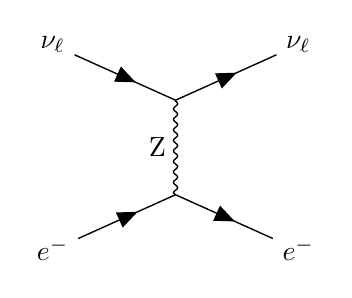
\begin{tikzpicture}[scale=1.2]
      \begin{feynhand}
        % vertices
        \vertex (vl1) at (0,0) {$\nu_\l$};
        \vertex (vl2) at (2.6,0) {$\nu_\l$};
        \vertex (a) at (1.3,-0.585);
        \vertex (b) at (1.3,-1.585);
        \vertex (e1) at (0,-2.17) {$e^-$};
        \vertex (e2) at (2.6,-2.17) {$e^-$};
        % propags
        \propag[fer] (vl1) to (a);
        \propag[fer] (a) to (vl2);
        \propag[bos] (a) to [edge label'=\(\mathrm{Z}\)] (b);
        \propag[fer] (e1) to (b);
        \propag[fer] (b) to (e2);
      \end{feynhand}
    \end{tikzpicture}
    \caption{Neutrino-Electron Scattering}\label{fig:t51}
  \end{figure}
  \begin{figure}[H]
    \centering
    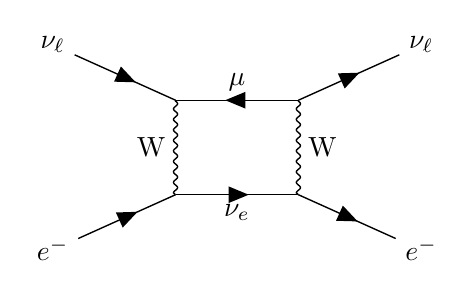
\begin{tikzpicture}[scale=1.2]
      \begin{feynhand}
        % vertices
        \vertex (vl1) at (0,0) {$\nu_\l$};
        \vertex (vl2) at (3.9,0) {$\nu_\l$};
        \vertex (a) at (1.3,-0.585);
        \vertex (b) at (1.3,-1.585);
        \vertex (c) at (2.6,-0.585);
        \vertex (d) at (2.6,-1.585);
        \vertex (e1) at (0,-2.17) {$e^-$};
        \vertex (e2) at (3.9,-2.17) {$e^-$};
        % propags
        \propag[fer] (vl1) to (a);
        \propag[fer] (c) to (vl2);
        \propag[fer] (e1) to (b);
        \propag[fer] (d) to (e2);
        % box
        \propag[bos] (a) to [edge label'=\(\mathrm{W}\)] (b);
        \propag[bos] (c) to [edge label=\(\mathrm{W}\)] (d);
        \propag[antfer] (a) to [edge label=\(\mu\)] (c);
        \propag[fer] (b) to [edge label'=\(\nu_e\)] (d);
      \end{feynhand}
    \end{tikzpicture}
    \caption{Neutrino-Electron Scattering at Higher Order}\label{fig:t52}
  \end{figure}
  \begin{enumerate}
  \item What is the matrix element for this process?
  \item Before doing any calculations explain which helicity combinations will give nonzero matrix element.
  \item Calculate the matrix element for each nonzero helicity combination.
  \item Calculate the spin-average matrix element squared.
  \item What is the differential cross section? Write the final result in terms of the vector and axial-vector couplings.
  \item For Phys 167B:\@ The first observation of the neutral current was seen at CERN in the 1970s\footnote{ \url{https://cerncourier.com/a/gargamelle-the-tale-of-a-giant-discovery/}}. How did researchers know it was a new type of interaction mediated by the $\mathrm{Z}$ boson instead of the diagram shown in Figure~\ref{fig:t52}?
  \end{enumerate}
\end{problem}
The diagram with momentum labels is seen in figure~\ref{fig:t53}, we can do calculations from there:
\begin{figure}[H]
  \centering
  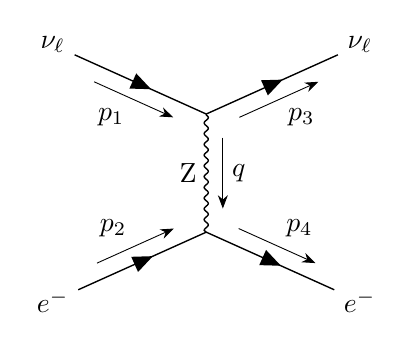
\begin{tikzpicture}[scale=1.5]
    \begin{feynhand}
      % vertices
      \vertex (vl1) at (0,0) {$\nu_\l$};
      \vertex (vl2) at (2.6,0) {$\nu_\l$};
      \vertex (a) at (1.3,-0.585);
      \vertex (b) at (1.3,-1.585);
      \vertex (e1) at (0,-2.17) {$e^-$};
      \vertex (e2) at (2.6,-2.17) {$e^-$};
      % propags
      \propag[fer, mom'=\(p_1\)] (vl1) to (a);
      \propag[fer, mom'=\(p_3\)] (a) to (vl2);
      \propag[bos, mom=\(q\)] (a) to [edge label'=\(\mathrm{Z}\)] (b);
      \propag[fer, mom=\(p_2\)] (e1) to (b);
      \propag[fer, mom=\(p_4\)] (b) to (e2);
    \end{feynhand}
    \end{tikzpicture}
  \caption{Neutrino-Electron Scattering, Momentum Labels}\label{fig:t53}
\end{figure}
We then get the matrix element by multiplying all the proper terms:
\begin{align*}
  -i\M&=\bar{u}(p_3)\qty[-i\frac{g_W}{\cos\theta_W}\gamma^\mu\frac12
  \qty(c_V^{(\nu)}-c_A^{(\nu)}\gamma^5)]u(p_1)\\
  &\times-i\frac{g_{\mu\nu}-q_\mu q_\nu/m_Z^2}{q^2-m^2_Z}\\
  &\times\bar{u}(p_4)\qty[-i\frac{g_W}{\cos\theta_W}\gamma^\nu\frac12
  \qty(c_V^{(e)}-c_A^{(e)}\gamma^5)]u(p_2)
\end{align*}
We will simplify this quite a bit, especially the propagator, turning it into a contact interaction and we can ignore the $q_\mu$ termm, as well as condense the $g_W/\cos\theta_W$ into $g_Z$:
\begin{align*}
  -i\M=i\frac{g_{\mu\nu}}{m^2_Z}
  &\times\bar{u}(p_3)\qty[-ig_Z\gamma^\mu\frac12
  \qty(c_V^{(\nu)}-c_A^{(\nu)}\gamma^5)]u(p_1)\\
  &\times\bar{u}(p_4)\qty[-ig_Z\gamma^\nu\frac12
  \qty(c_V^{(e)}-c_A^{(e)}\gamma^5)]u(p_2)
\end{align*}
Simplifying a bit:
\begin{align*}
  -i\M&=-i\frac{g_Z^2}{m_Z^2}g_{\mu\nu}
  \qty[\bar{u}(p_3)\gamma^\mu\frac12\qty(c_V^{(\nu)}-c_A^{(\nu)}\gamma^5)u(p_1)]
  \qty[\bar{u}(p_4)\gamma^\nu\frac12\qty(c_V^{(e)}-c_A^{(e)}\gamma^5)u(p_2)]
\end{align*}
Hence the bare matrix element is:
\begin{equation}
  \label{eq:t51}
  \boxed{
    \begin{aligned}
      \M=\frac{g_Z^2}{m_Z^2}g_{\mu\nu}
      &\times\qty[\bar{u}(p_3)\gamma^\mu
      \frac12\qty(c_V^{(\nu)}-c_A^{(\nu)}\gamma^5)u(p_1)]\\
      &\times \qty[\bar{u}(p_4)\gamma^\nu
      \frac12\qty(c_V^{(e)}-c_A^{(e)}\gamma^5)u(p_2)]
  \end{aligned}}
\end{equation}
To see which helicity combinations are nonzero, it is helpful to rewrite the currents in terms of the chiral projectors and the $c_L/c_R$ coefficients:
\begin{align*}
  j^\mu_{(\nu)}&=\qty[\bar{u}(p_3)\gamma^\mu
  \frac12\qty(c_V^{(\nu)}-c_A^{(\nu)}\gamma^5)u(p_1)]\\
  &=c_L^{(\nu)}\bar{u}(p_3)\gamma^\mu P_L u(p_1)
  +c_R^{(\nu)}\bar{u}(p_3)\gamma^\mu P_R u(p_1)\\
  j^\nu_{(e)}&=\qty[\bar{u}(p_4)\gamma^\nu
  \frac12\qty(c_V^{(e)}-c_A^{(e)}\gamma^5)u(p_2)]\\
  &=c_L^{(e)}\bar{u}(p_4)\gamma^\nu P_L u(p_2)
  +c_R^{(e)}\bar{u}(p_4)\gamma^\nu P_R u(p_2)
\end{align*}
We can immediately get rid of the RH neutrino contributions since only LH neutrinos participate in the neutral current interaction:
\begin{align*}
  j^\mu_{(\nu)}=c_L^{(\nu)}\bar{u}_\downarrow(p_3)\gamma^\mu u_\downarrow(p_1)
\end{align*}
And there is no constraint on the handedness of the electron, so we have two nonzero matrix elements, $\M_{LR}$ and $\M_{LL}$:
\begin{equation}
  \label{eq:t52}
  \boxed{
    \M_{RL}=\M_{RR}=0
  }
\end{equation}
Using the ultra-relativistic limit, we have the following spinors:
\begin{gather*}
  % u_\uparrow(p_1)=\sqrt{E}\pmqty{1\\0\\1\\0}\quad
  u_\downarrow(p_1)=\sqrt{E}\pmqty{0\\1\\0\\-1}\quad
  u_\downarrow(p_3)=\sqrt{E}\pmqty{-s\\c\\s\\-c}\\
  u_\uparrow(p_2)=\sqrt{E}\pmqty{0\\-1\\0\\-1}\quad
  u_\downarrow(p_2)=\sqrt{E}\pmqty{-1\\0\\1\\0}\\
  % u_\uparrow(p_3)=\sqrt{E}\pmqty{c\\s\\c\\s}\quad
  u_\uparrow(p_4)=\sqrt{E}\pmqty{s\\-c\\s\\-c}\quad
  u_\downarrow(p_4)=\sqrt{E}\pmqty{-c\\-s\\c\\s}
\end{gather*}
Where $s=\sin\theta/2$ and $c=\cos\theta/2$ and $E$ is the energy in the center of mass frame.

From here we can calculate the currents, finding that:
\begin{align*}
  j^\mu_{(\nu)}&=2E(c,s,-is,c)\\
  j^\nu_{(e),L}&=\bar{u}_\downarrow(p_4)\gamma^\nu u_\downarrow(p_2)
  =2E(c,-s,-is,-c)\\
  j^\nu_{(e),R}&=\bar{u}_\uparrow(p_4)\gamma^\nu u_\uparrow(p_2)
  =2E(c,-s,+is,-c)
\end{align*}
We then form the dot products:
\begin{align*}
  j_{(\nu)}\vdot j_{(e),L}
  &=4E^2(c^2+s^2+s^2+c^2)=8E^2\\
  j_{(\nu)}\vdot j_{(e),R}
  &=8E^2c^2
\end{align*}
We can reduce this by writing $E=\sqrt{s}/2$ and writing $c^2=\frac12(1+\cos\theta)$:
\begin{align*}
  j_{(\nu)}\vdot j_{(e),L}
  &=2s\\
  j_{(\nu)}\vdot j_{(e),R}
  &=s(1+\cos\theta)
\end{align*}
Hence the matrix elements are:
\begin{equation}
  \label{eq:t53}
  \boxed{
    \begin{aligned}
      \M_{LL}&=\frac{2g_Z^2s}{m_Z^2}c^{(\nu)}_L c^{(e)}_L\\
      \M_{LR}&=\frac{g_Z^2s}{m_Z^2}
      c_L^{(\nu)}c_R^{(e)}(1+\cos\theta)
    \end{aligned}
  }
\end{equation}
We can then average over the two spin states of the electron:
\begin{align*}
  \ev{\abs{\M}^2}&=\frac12
  \qty(\abs{\M_{LL}}^2+\abs{\M_{LR}}^2)\\
  &=\frac12\frac{g_Z^4s^2}{m_Z^4}{(c_L^{(\nu)})}^2
  \qty(4{(c_R^{(e)})}^2+{(c_R^{(e)})}^2{(1+\cos\theta)}^2)\\
  &=\frac12\frac{g_Z^4s^2}{m_Z^4}{\qty(\frac12)}^2
  \qty(4{(c_L^{(e)})}^2+{(c_R^{(e)})}^2{(1+\cos\theta)}^2)
\end{align*}
Some simplifications give our final answer for the spin averaged matrix element
\begin{equation}
  \label{eq:t54}
  \boxed{\ev{\abs{\M}^2}=\frac{g_Z^4s^2}{2m_Z^4}
  \qty({(c_L^{(e)})}^2+{(c_R^{(e)}/2)}^2{(1+\cos\theta)}^2)}
\end{equation}
The differential cross section is then given by the formula from the book
\begin{thebook}
  The expression for the differential cross section for the process $a+b\to c+d$ in the center-of-mass frame is
  \begin{align*}
    \dv{\sigma}{\Omega}=\frac1{64\pi^2s}\frac{p_f^*}{p_i^*}\abs{\M_{fi}}^2
  \end{align*}
\end{thebook}
We are using the ultra-relativistic limit so the initial and final momenta are the same, giving the differential cross section as:
\begin{align*}
  \dv{\sigma}{\Omega}=\frac{g_Z^4s}{128m_Z^4}
  \qty({(c_L^{(e)})}^2+{(c_R^{(e)}/2)}^2{(1+\cos\theta)}^2)
\end{align*}
All that remains is the replacement to the $c_V/c_A$ couplings once more:
\begin{equation}
  \label{eq:t55}
  \boxed{
    \dv{\sigma}{\Omega}=\frac{g_Z^4s}{2048m_Z^4}\qty(
    4{\qty(c_V^{(e)}+c_A^{(e)})}^2
    +{\qty(c_V^{(e)}-c_A^{(e)})}^2{(1+\cos\theta)}^2)
  }
\end{equation}

The type of diagram seen in figure~\ref{fig:t52} is highly suppressed, and the matrix element would be $\order{g_W^4}$ as opposed to our process which is $\order{g_Z^2}$, so with higher statistics it is much less likely to observe these events.
\end{document}